\newcommand{\heatmapwidth}{0.495\textwidth}
\newcommand{\heatmapheight}{4cm}
\begin{figure}[H]
	\centering
	\begin{subfigure}[b]{\heatmapwidth}
        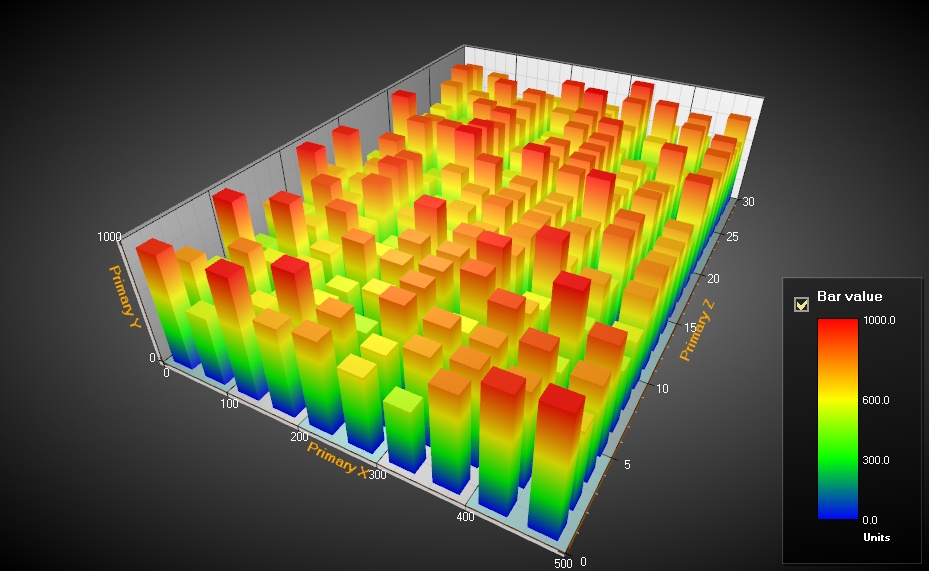
\includegraphics[width=\textwidth,height=\heatmapheight]{images/heat-map-1}
        \caption{A heat map of financial data. \protect\footnotemark}
        \label{fig:heat_map_financial}
    \end{subfigure}
    \begin{subfigure}[b]{\heatmapwidth}
        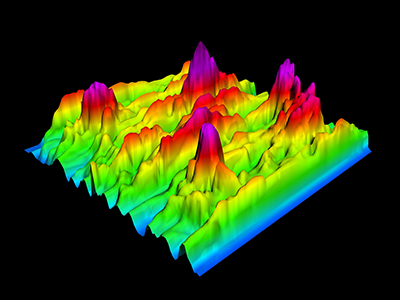
\includegraphics[width=\textwidth,height=\heatmapheight]{images/heat-map-2}
        \caption{A heat map of electroencephalogram. \protect\footnotemark}
        \label{fig:heat_map_eeg}
    \end{subfigure}
	\caption{Two different representations of a heat map.}
	\subfigcaptionskip
	\label{fig:heat_maps}
\end{figure}

\addtocounter{footnote}{-2}
\stepcounter{footnote}\footnotetext{\bibentry{tuomainen2014financial}}
\stepcounter{footnote}\footnotetext{\bibentry{fuchs2006physiological}}
